%%%%%%%%%%%%%%%%%%%%%%%%%%%%%%%%%%%%%%%%%
% Jacobs Landscape Poster
% LaTeX Template
% Version 1.0 (29/03/13)
% This template has been downloaded from:
% http://www.LaTeXTemplates.com
%
% Created by:
% Computational Physics and Biophysics Group, Jacobs University
% https://teamwork.jacobs-university.de:8443/confluence/display/CoPandBiG/LaTeX+Poster
% 
% Further modified by:
% Nathaniel Johnston (nathaniel@njohnston.ca)
%
% This template has been downloaded from:
% http://www.LaTeXTemplates.com
%
% License:
% CC BY-NC-SA 3.0 (http://creativecommons.org/licenses/by-nc-sa/3.0/)
%
%%%%%%%%%%%%%%%%%%%%%%%%%%%%%%%%%%%%%%%%%

%----------------------------------------------------------------------------------------
%	PACKAGES AND OTHER DOCUMENT CONFIGURATIONS
%----------------------------------------------------------------------------------------

\documentclass[final]{beamer}

\usepackage[scale=1.24]{beamerposter} % Use the beamerposter package for laying out the poster
\usepackage{cite}
\usepackage{amsmath,amssymb,amsfonts}
\usepackage{algorithmic}
\usepackage{graphicx}
\usepackage{textcomp}
\usepackage{xcolor}

\usetheme{confposter} % Use the confposter theme supplied with this template

\setbeamercolor{block title}{fg=ngreen,bg=white} % Colors of the block titles
\setbeamercolor{block body}{fg=black,bg=white} % Colors of the body of blocks
\setbeamercolor{block alerted title}{fg=white,bg=dblue!70} % Colors of the highlighted block titles
\setbeamercolor{block alerted body}{fg=black,bg=dblue!10} % Colors of the body of highlighted blocks
% Many more colors are available for use in beamerthemeconfposter.sty

%-----------------------------------------------------------
% Define the column widths and overall poster size
% To set effective sepwid, onecolwid and twocolwid values, first choose how many columns you want and how much separation you want between columns
% In this template, the separation width chosen is 0.024 of the paper width and a 4-column layout
% onecolwid should therefore be (1-(# of columns+1)*sepwid)/# of columns e.g. (1-(4+1)*0.024)/4 = 0.22
% Set twocolwid to be (2*onecolwid)+sepwid = 0.464
% Set threecolwid to be (3*onecolwid)+2*sepwid = 0.708

\newlength{\sepwid}
\newlength{\onecolwid}
\newlength{\twocolwid}
\newlength{\threecolwid}
\setlength{\paperwidth}{70in}  % 70in~5.83feet; A0 width: 46.8in
\setlength{\paperheight}{38in} % 38in~3.17feet; A0 height: 33.1in
\setlength{\sepwid}{0.024\paperwidth} % Separation width (white space) between columns
\setlength{\onecolwid}{0.22\paperwidth} % Width of one column
\setlength{\twocolwid}{0.464\paperwidth} % Width of two columns
\setlength{\threecolwid}{0.708\paperwidth} % Width of three columns
\setlength{\topmargin}{-0.5in} % Reduce the top margin size
%-----------------------------------------------------------

\usepackage{graphicx}  % Required for including images

\usepackage{booktabs} % Top and bottom rules for tables

%----------------------------------------------------------------------------------------
%	TITLE SECTION 
%----------------------------------------------------------------------------------------

\title{A Hybrid Approach to Scientific Software Package Management \\ on a High-Performance Computing Cluster} % Poster title

\author{Qiyang Hu, Shao-Ching Huang} % Author(s)

\institute{Institute for Digital Research and Education, University of California, Los Angeles (UCLA)} % Institution(s)

%----------------------------------------------------------------------------------------

\begin{document}

\addtobeamertemplate{block end}{}{\vspace*{2ex}} % White space under blocks
\addtobeamertemplate{block alerted end}{}{\vspace*{2ex}} % White space under highlighted (alert) blocks

\setlength{\belowcaptionskip}{2ex} % White space under figures
\setlength\belowdisplayshortskip{2ex} % White space under equations

\begin{frame}[t] % The whole poster is enclosed in one beamer frame

\begin{columns}[t] % The whole poster consists of three major columns, the second of which is split into two columns twice - the [t] option aligns each column's content to the top

\begin{column}{\sepwid}\end{column} % Empty spacer column

\begin{column}{\onecolwid} % The first column

%----------------------------------------------------------------------------------------
%	OBJECTIVES
%----------------------------------------------------------------------------------------

\begin{alertblock}{Abstract}

We present a new approach for managing the scientific packages in an HPC cluster environment, particularly suitable in a research university environment that has a diverse user base.
The goal is to minimize the HPC operational team's burden of installing and maintaining a large number of software packages to support a broadband spectrum of university research.
We propose a hybridizing management method that can harness the power of modern software management frameworks and the flexibility of in-house, or ``manual'', installation sources, and at the same time present a coherent view to the end users. Spack~\cite{gamblin:15} was used in this work. Our hybrid approach is applicable to using other framework tools. The manipulation of environment module files and the typical workflow are illustrated, followed by discussions.


\end{alertblock}

%----------------------------------------------------------------------------------------
%	INTRODUCTION
%----------------------------------------------------------------------------------------

\begin{block}{Introduction}

\hspace{2em}Having to install and maintain a large number of software packages to support the broadband spectrum of university research motivates the use of a software installation framework, such as EasyBuild\cite{geimer:14} or Spack\cite{gamblin:15}, to automate the processes and thus lessen the burden on HPC operational teams. 
However, challenges arise when the framework has to be integrated with in-house package installation practices already existed. In practice, the in-house installation component is required because not all packages can be satisfactorily managed within a software management framework.

\hspace{2em}In this work, we propose a practical approach for HPC cluster operational teams to manage software packages by hybridizing the framework and manual-based installation methods. 
From a software design point of view, our central idea is to add a layer above the existing software management frameworks, where a workflow is introduced to manage applications built either by the framework or by manual installation to enable flexible customization, complying to the existing structure of the HPC cluster environment.
In this paper, we adopt Spack as the package management framework. The proposed approach is applicable to using other software management frameworks. We consider the deployment of the hybrid approach on UCLA Hoffman2 Cluster where an in-house package installation structure already exists.
It should be noted that the framework-installed and manually-installed packages are kept separate by design, so it will allow future changes of the HPC environment, including the possibility of adopting another installation framework.
A main contribution of this work is a noble way to manipulate and re-organize the environment modules and offer a practical, automated and script-able workflow to build and maintain the packages, and to provide a coherent view to end users.

\end{block}

%------------------------------------------------

%== \begin{figure}
%== \includegraphics[width=0.8\linewidth]{placeholder.jpg}
%== \caption{Figure caption}
%== \end{figure}

%----------------------------------------------------------------------------------------

\end{column} % End of the first column


%----------------------------------------------------------------------------------------

\begin{column}{\sepwid}\end{column} % Empty spacer column

\begin{column}{\onecolwid} % Second column 

%----------------------------------------------------------------------------------------
%	Modulefile Structure Customization
%----------------------------------------------------------------------------------------


\begin{block}{Modulefile Structure Customization}

Adding a flexible management layer on top of framework requires traversing the module file structure generated by the software management framework.
Based on our experience, also motivated by the operation of other large-scale HPC clusters (e.g. TACC Stampede), we first propose the module files to be organized in a simple structure as shown in Figure below, where the MPI level is nested in the compiler level. 
The versions of compilers and MPIs follow the convention in Spack. 

\vspace{0.75em}
\begin{figure}[htbp]
  \centerline{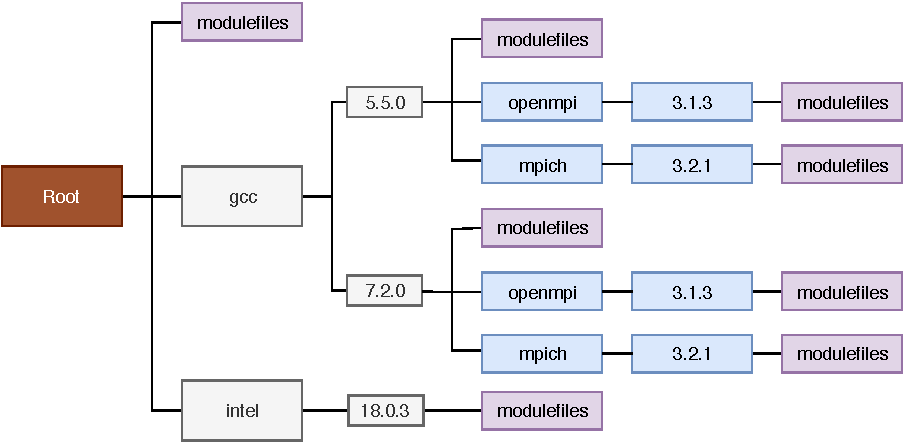
\includegraphics[width=0.9\linewidth]{figures/h2_new_hier}}
  \caption{Newly defined hierarchical structure of module files in Hoffman2}
  \label{fig:h2_new_hier}
\end{figure}


\end{block}


%----------------------------------------------------------------------------------------
%	Using JSON Files
%----------------------------------------------------------------------------------------

\vspace{-1em}
\begin{block}{Using JSON For Interfacing with Support}

We use JSON to express the information of the packages that our HPC operational team will support, i.e. visible to end users. An example of a JSON file is listed below:

\texttt{
\{  "bowtie2": \{ \\
\qquad \qquad         "name\_in\_spack": "bowtie2", \\
\qquad \qquad         "version": [ \\
\qquad \qquad \qquad             "2.3.4.1-gcc-7.2.0",\\
\qquad \qquad \qquad             "2.3.4.1-gcc-5.5.0" \\
\qquad \qquad         ], \\
\qquad \qquad         "default": "2.3.4.1" \\
\qquad     \}, \\
\}, \\
}

where the main name in the json object pair is the application name preferred by system admins. The \texttt{name\_in\_spack} is the name used in Spack. It can be blank if there is no cooresponding one in Spack. The \texttt{version} keeps the application version information and the corresponding compilers. The default version that will be shown or selected by the \texttt{Lmod} system.

\end{block}

\end{column} % End of 2nd column
%----------------------------------------------------------------------------------------


\begin{column}{\sepwid}\end{column} % Empty spacer column

\begin{column}{\onecolwid} % 3rd column

%----------------------------------------------------------------------------------------
%	Modulefile Hybridization 
%----------------------------------------------------------------------------------------

\begin{block}{Hybridization of Modulefiles}

Our approach takes advantage of Spack's capability of generating both flat and hierarchical module files by enabling them in modules.yaml configuration file. Figure below shows our module filtering process which will do a few additional steps of:

\setlength{\leftmargini}{9.5cm}
\setlength{\leftmarginii}{9.5cm}
\begin{itemize}
    \item Calling \texttt{tcl2lua.tcl} script
    \item Pre-pending \texttt{MODULEPATH} 
    \item Adding \texttt{family} 
    \item Generating \texttt{.version} file
\end{itemize}

\vspace{0.75em}
\begin{figure}
  \centerline{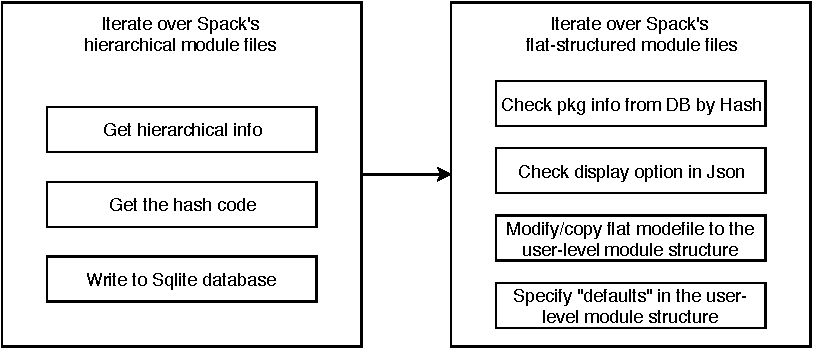
\includegraphics[width=0.8\linewidth]{figures/modulefilter_flowchart}}
  \caption{Flowchart for the python script to generate the newly defined module file structures}
\end{figure}

\end{block}

%----------------------------------------------------------------------------------------
%	Workflow
%----------------------------------------------------------------------------------------

\vspace{-1em}
\begin{block}{Operational Workflow}

\begin{figure}
  \centerline{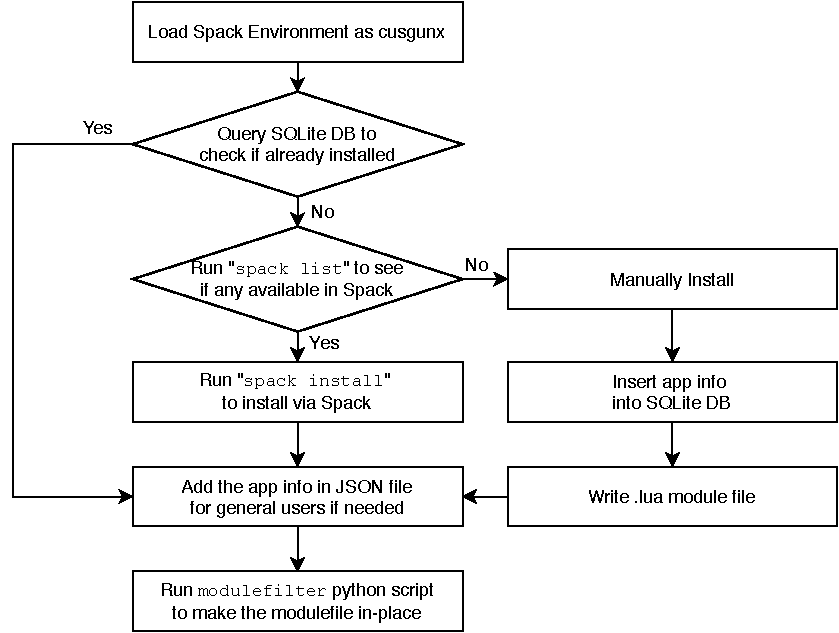
\includegraphics[width=0.8\linewidth]{figures/spack_h2_hybrid_flow}}
  \caption{Workflow to hybridize the Spack-installed and manually-installed packages}
\end{figure}


\end{block}

\end{column} % End of the third column
%----------------------------------------------------------------------------------------


\begin{column}{\sepwid}\end{column} % Empty spacer column

\begin{column}{\onecolwid} % The fourth column

%----------------------------------------------------------------------------------------
%	SUMMARY
%----------------------------------------------------------------------------------------

\begin{block}{Summary}

In this work we proposed an approach to hybridize the software management framework and the traditional manual package management. 
The design adds a layer on top of the standard package management framework expecting to take advantage of the powerfule framework while maintaining the management flexibility for manual installations and the customizable HPC user interface. 
With the definition of a module file structure in the HPC cluster environment, the workflow is able to process, filter and integrate the module files from two independent sources (i.e. framework-based and manual-based) to any target modulefile presentation. 

\end{block}

%----------------------------------------------------------------------------------------
%	ADDITIONAL INFORMATION
%----------------------------------------------------------------------------------------

\begin{block}{Additional Information}

Our work has been uploaded to the gitlab repo:
\begin{itemize}
\item \href{https://gitlab.idre.ucla.edu/hoffman2/modulefile-processing}{https://gitlab.idre.ucla.edu/hoffman2/modulefile-processing}
\end{itemize}

\end{block}

%----------------------------------------------------------------------------------------
%	REFERENCES
%----------------------------------------------------------------------------------------

\begin{block}{References}

\nocite{*} % Insert publications even if they are not cited in the poster
\small{\bibliographystyle{unsrt}
%\bibliography{sample}\vspace{0.75in}}

\begin{thebibliography}{00}
\bibitem{geimer:14} Markus Geimer, Kenneth Hoste, Robert McLay. ``Modern Scientific Software Management Using EasyBuild and Lmod'' HUST '14: Proceedings of the First International Workshop on HPC User Support Tools, page 41-51, November 2014.
\bibitem{gamblin:15} Todd Gamblin, Matthew LeGendre, Michael R. Collette, Gregory L. Lee, Adam Moody, Bronis R. de Supinski, and Scott Futral. ``The spack package manager: bringing order to hpc software chaos,'' SC ’15 Proceedings of the International Conference for High Performance Computing, Networking, Storage and Analysis, 2015.
\bibitem{mclay:11} R. McLay, K. W. Schulz, W. L. Barth, and T. Minyard. ``Best practices for the deployment and management of production hpc clusters,'' In SC ’11 In State of the Practice Reports, page 9:1–9:11, 2011.
\bibitem{spack:20} \href{https://spack.readthedocs.io/en/latest}{https://spack.readthedocs.io/en/latest}
%== \bibitem{geimer:14} Markus Geimer, et al. HUST '14: Proceedings of the First International Workshop on HPC User Support Tools, page 41-51, November 2014.
%== \bibitem{gamblin:15} Todd Gamblin, et al. SC ’15 Proceedings of the International Conference for High Performance Computing, Networking, Storage and Analysis, 2015.
%== \bibitem{mclay:11} R. McLay, et al.  In SC ’11 In State of the Practice Reports, page 9:1–9:11, 2011.
%== \bibitem{spack:20} \href{https://spack.readthedocs.io/en/latest}{https://spack.readthedocs.io/en/latest}
%%\bibitem{gitlabrepo} \href{https://gitlab.idre.ucla.edu/hoffman2/modulefile-processing}{https://gitlab.idre.ucla.edu/hoffman2/modulefile-processing}
\end{thebibliography}
}

\end{block}

%== %----------------------------------------------------------------------------------------
%== %	ACKNOWLEDGEMENTS
%== %----------------------------------------------------------------------------------------
%== 
%== \setbeamercolor{block title}{fg=red,bg=white} % Change the block title color
%== 
%== \begin{block}{Acknowledgements}
%== 
%== \small{\rmfamily{Nam mollis tristique neque eu luctus. Suspendisse rutrum congue nisi sed convallis. Aenean id neque dolor. Pellentesque habitant morbi tristique senectus et netus et malesuada fames ac turpis egestas.}} \\
%== 
%== \end{block}

%----------------------------------------------------------------------------------------
%	CONTACT INFORMATION
%----------------------------------------------------------------------------------------

\setbeamercolor{block alerted title}{fg=black,bg=norange} % Change the alert block title colors
\setbeamercolor{block alerted body}{fg=black,bg=white} % Change the alert block body colors

\begin{alertblock}{Contact Information}

\begin{itemize}
\item Email: \href{mailto:huqy@idre.ucla.edu}{huqy@idre.ucla.edu}, \href{mailto:schuang@idre.ucla.edu}{schuang@idre.ucla.edu}
\item Phone: +1-(310)-825-2011, +1-(310)-825-4874
\end{itemize}

\end{alertblock}

\begin{center}
\begin{tabular}{ccc}

\includegraphics[width=0.4\linewidth]{figures/ucla_logo.jpg} & \hfill & 
\includegraphics[width=0.4\linewidth]{figures/idre_logo.jpg}
\end{tabular}
\end{center}

\end{column} % End of the fourth column
%----------------------------------------------------------------------------------------


\end{columns} % End of all the columns in the poster

\end{frame} % End of the enclosing frame

\end{document}

